\documentclass[crop, tikz]{standalone}
\usepackage{tikz}

\usetikzlibrary{decorations.pathmorphing,positioning}

\begin{document}
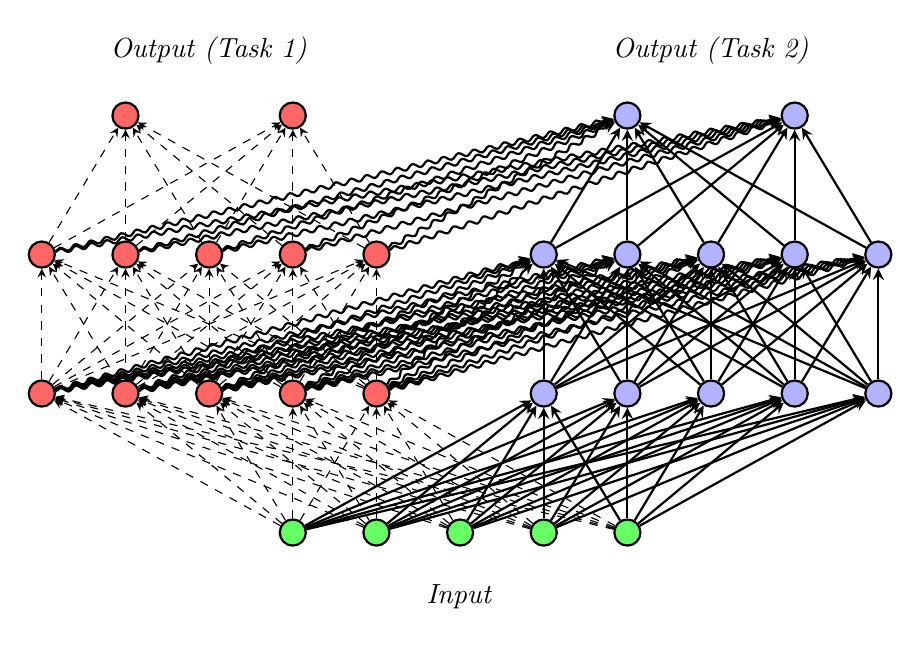
\begin{tikzpicture}
	\node[circle, draw, thick, fill=green!60] (i1) {};
	\node[circle, draw, thick, fill=green!60, right=2em of i1] (i2) {};
	\node[circle, draw, thick, fill=green!60, right=2em of i2] (i3) {};
	\node[circle, draw, thick, fill=green!60, left=2em of i1] (i4) {};
	\node[circle, draw, thick, fill=green!60, left=2em of i4] (i5) {};
	
	\node[below=1em of i1] (lab1) {\emph{Input}};
	
	\node[circle, draw, thick, fill=red!60,above=4em of i4] (h1) {};
	\node[circle, draw, thick, fill=red!60,left=2em of h1] (h2) {};
	\node[circle, draw, thick, fill=red!60, left=2em of h2] (h3) {};
	\node[circle, draw, thick, fill=red!60,left=2em of h3] (h4) {};
	\node[circle, draw, thick, fill=red!60, left=2em of h4] (h5) {};
	
	\node[circle, draw, thick, fill=red!60,above=4em of h1] (hh1) {};
	\node[circle, draw, thick, fill=red!60,above=4em of h2] (hh2) {};
	\node[circle, draw, thick, fill=red!60,above=4em of h3] (hh3) {};
	\node[circle, draw, thick, fill=red!60,above=4em of h4] (hh4) {};
	\node[circle, draw, thick, fill=red!60,above=4em of h5] (hh5) {};
	
	\node[circle, draw, thick, fill=red!60,above=4em of hh2] (o1) {};
	\node[circle, draw, thick, fill=red!60,above=4em of hh4] (o2) {};
	
	\draw[-stealth, thin, dashed] (i1) -- (h1);
	\draw[-stealth, thin, dashed] (i1) -- (h2);
	\draw[-stealth, thin, dashed] (i1) -- (h3);
	\draw[-stealth, thin, dashed] (i1) -- (h4);
	\draw[-stealth, thin, dashed] (i1) -- (h5);
	\draw[-stealth, thin, dashed] (i2) -- (h1);
	\draw[-stealth, thin, dashed] (i2) -- (h2);
	\draw[-stealth, thin, dashed] (i2) -- (h3);
	\draw[-stealth, thin, dashed] (i2) -- (h4);
	\draw[-stealth, thin, dashed] (i2) -- (h5);
	\draw[-stealth, thin, dashed] (i3) -- (h1);
	\draw[-stealth, thin, dashed] (i3) -- (h2);
	\draw[-stealth, thin, dashed] (i3) -- (h3);
	\draw[-stealth, thin, dashed] (i3) -- (h4);
	\draw[-stealth, thin, dashed] (i3) -- (h5);
	\draw[-stealth, thin, dashed] (i4) -- (h1);
	\draw[-stealth, thin, dashed] (i4) -- (h2);
	\draw[-stealth, thin, dashed] (i4) -- (h3);
	\draw[-stealth, thin, dashed] (i4) -- (h4);
	\draw[-stealth, thin, dashed] (i4) -- (h5);
	\draw[-stealth, thin, dashed] (i5) -- (h1);
	\draw[-stealth, thin, dashed] (i5) -- (h2);
	\draw[-stealth, thin, dashed] (i5) -- (h3);
	\draw[-stealth, thin, dashed] (i5) -- (h4);
	\draw[-stealth, thin, dashed] (i5) -- (h5);
	
	\draw[-stealth, thin, dashed] (h1) -- (hh1);
	\draw[-stealth, thin, dashed] (h1) -- (hh2);
	\draw[-stealth, thin, dashed] (h1) -- (hh3);
	\draw[-stealth, thin, dashed] (h1) -- (hh4);
	\draw[-stealth, thin, dashed] (h1) -- (hh5);
	\draw[-stealth, thin, dashed] (h2) -- (hh1);
	\draw[-stealth, thin, dashed] (h2) -- (hh2);
	\draw[-stealth, thin, dashed] (h2) -- (hh3);
	\draw[-stealth, thin, dashed] (h2) -- (hh4);
	\draw[-stealth, thin, dashed] (h2) -- (hh5);
	\draw[-stealth, thin, dashed] (h3) -- (hh1);
	\draw[-stealth, thin, dashed] (h3) -- (hh2);
	\draw[-stealth, thin, dashed] (h3) -- (hh3);
	\draw[-stealth, thin, dashed] (h3) -- (hh4);
	\draw[-stealth, thin, dashed] (h3) -- (hh5);
	\draw[-stealth, thin, dashed] (h4) -- (hh1);
	\draw[-stealth, thin, dashed] (h4) -- (hh2);
	\draw[-stealth, thin, dashed] (h4) -- (hh3);
	\draw[-stealth, thin, dashed] (h4) -- (hh4);
	\draw[-stealth, thin, dashed] (h4) -- (hh5);
	\draw[-stealth, thin, dashed] (h5) -- (hh1);
	\draw[-stealth, thin, dashed] (h5) -- (hh2);
	\draw[-stealth, thin, dashed] (h5) -- (hh3);
	\draw[-stealth, thin, dashed] (h5) -- (hh4);
	\draw[-stealth, thin, dashed] (h5) -- (hh5);
	
	
	\draw[-stealth, thin, dashed] (hh1) -- (o1);
	\draw[-stealth, thin, dashed] (hh1) -- (o2);
	\draw[-stealth, thin, dashed] (hh2) -- (o1);
	\draw[-stealth, thin, dashed] (hh2) -- (o2);
	\draw[-stealth, thin, dashed] (hh3) -- (o1);
	\draw[-stealth, thin, dashed] (hh3) -- (o2);
	\draw[-stealth, thin, dashed] (hh4) -- (o1);
	\draw[-stealth, thin, dashed] (hh4) -- (o2);
	\draw[-stealth, thin, dashed] (hh5) -- (o1);
	\draw[-stealth, thin, dashed] (hh5) -- (o2);
	
	\node[above=6em of hh3] (lab1) {\emph{Output (Task 1)}};
	
	
	\node[circle, draw, thick, fill=blue!30,above=4em of i2] (ih1) {};
	\node[circle, draw, thick, fill=blue!30,right=2em of ih1] (ih2) {};
	\node[circle, draw, thick, fill=blue!30,right=2em of ih2] (ih3) {};
	\node[circle, draw, thick, fill=blue!30,right=2em of ih3] (ih4) {};
	\node[circle, draw, thick, fill=blue!30,right=2em of ih4] (ih5) {};
	
	\node[circle, draw, thick, fill=blue!30,above=4em of ih1] (ihh1) {};
	\node[circle, draw, thick, fill=blue!30,above=4em of ih2] (ihh2) {};
	\node[circle, draw, thick, fill=blue!30,above=4em of ih3] (ihh3) {};
	\node[circle, draw, thick, fill=blue!30,above=4em of ih4] (ihh4) {};
	\node[circle, draw, thick, fill=blue!30,above=4em of ih5] (ihh5) {};
	
	\node[circle, draw, thick, fill=blue!30,above=4em of ihh2] (io1) {};
	\node[circle, draw, thick, fill=blue!30,above=4em of ihh4] (io2) {};
	
	\node[above=6em of ihh3] (lab1) {\emph{Output (Task 2)}};
	
	\draw[-stealth, thick] (i1) -- (ih1);
	\draw[-stealth, thick] (i1) -- (ih2);
	\draw[-stealth, thick] (i1) -- (ih3);
	\draw[-stealth, thick] (i1) -- (ih4);
	\draw[-stealth, thick] (i1) -- (ih5);
	\draw[-stealth, thick] (i2) -- (ih1);
	\draw[-stealth, thick] (i2) -- (ih2);
	\draw[-stealth, thick] (i2) -- (ih3);
	\draw[-stealth, thick] (i2) -- (ih4);
	\draw[-stealth, thick] (i2) -- (ih5);
	\draw[-stealth, thick] (i3) -- (ih1);
	\draw[-stealth, thick] (i3) -- (ih2);
	\draw[-stealth, thick] (i3) -- (ih3);
	\draw[-stealth, thick] (i3) -- (ih4);
	\draw[-stealth, thick] (i3) -- (ih5);
	\draw[-stealth, thick] (i4) -- (ih1);
	\draw[-stealth, thick] (i4) -- (ih2);
	\draw[-stealth, thick] (i4) -- (ih3);
	\draw[-stealth, thick] (i4) -- (ih4);
	\draw[-stealth, thick] (i4) -- (ih5);
	\draw[-stealth, thick] (i5) -- (ih1);
	\draw[-stealth, thick] (i5) -- (ih2);
	\draw[-stealth, thick] (i5) -- (ih3);
	\draw[-stealth, thick] (i5) -- (ih4);
	\draw[-stealth, thick] (i5) -- (ih5);
	
	\draw[-stealth, thick] (ih1) -- (ihh1);
	\draw[-stealth, thick] (ih1) -- (ihh2);
	\draw[-stealth, thick] (ih1) -- (ihh3);
	\draw[-stealth, thick] (ih1) -- (ihh4);
	\draw[-stealth, thick] (ih1) -- (ihh5);
	\draw[-stealth, thick] (ih2) -- (ihh1);
	\draw[-stealth, thick] (ih2) -- (ihh2);
	\draw[-stealth, thick] (ih2) -- (ihh3);
	\draw[-stealth, thick] (ih2) -- (ihh4);
	\draw[-stealth, thick] (ih2) -- (ihh5);
	\draw[-stealth, thick] (ih3) -- (ihh1);
	\draw[-stealth, thick] (ih3) -- (ihh2);
	\draw[-stealth, thick] (ih3) -- (ihh3);
	\draw[-stealth, thick] (ih3) -- (ihh4);
	\draw[-stealth, thick] (ih3) -- (ihh5);
	\draw[-stealth, thick] (ih4) -- (ihh1);
	\draw[-stealth, thick] (ih4) -- (ihh2);
	\draw[-stealth, thick] (ih4) -- (ihh3);
	\draw[-stealth, thick] (ih4) -- (ihh4);
	\draw[-stealth, thick] (ih4) -- (ihh5);
	\draw[-stealth, thick] (ih5) -- (ihh1);
	\draw[-stealth, thick] (ih5) -- (ihh2);
	\draw[-stealth, thick] (ih5) -- (ihh3);
	\draw[-stealth, thick] (ih5) -- (ihh4);
	\draw[-stealth, thick] (ih5) -- (ihh5);
	
	\draw[-stealth, thick] (ihh1) -- (io1);
	\draw[-stealth, thick] (ihh1) -- (io2);
	\draw[-stealth, thick] (ihh2) -- (io1);
	\draw[-stealth, thick] (ihh2) -- (io2);
	\draw[-stealth, thick] (ihh3) -- (io1);
	\draw[-stealth, thick] (ihh3) -- (io2);
	\draw[-stealth, thick] (ihh4) -- (io1);
	\draw[-stealth, thick] (ihh4) -- (io2);
	\draw[-stealth, thick] (ihh5) -- (io1);
	\draw[-stealth, thick] (ihh5) -- (io2);
	
	
	\draw[-stealth, thick, decoration={snake, pre length=0.01mm, segment length=2mm, amplitude=0.3mm, post length=1.5mm}, decorate,] (h1) -- (ihh1);
	\draw[-stealth, thick, decoration={snake, pre length=0.01mm, segment length=2mm, amplitude=0.3mm, post length=1.5mm}, decorate,] (h1) -- (ihh2);
	\draw[-stealth, thick, decoration={snake, pre length=0.01mm, segment length=2mm, amplitude=0.3mm, post length=1.5mm}, decorate,] (h1) -- (ihh3);
	\draw[-stealth, thick, decoration={snake, pre length=0.01mm, segment length=2mm, amplitude=0.3mm, post length=1.5mm}, decorate,] (h1) -- (ihh4);
	\draw[-stealth, thick, decoration={snake, pre length=0.01mm, segment length=2mm, amplitude=0.3mm, post length=1.5mm}, decorate,] (h1) -- (ihh5);
	\draw[-stealth, thick, decoration={snake, pre length=0.01mm, segment length=2mm, amplitude=0.3mm, post length=1.5mm}, decorate,] (h2) -- (ihh1);
	\draw[-stealth, thick, decoration={snake, pre length=0.01mm, segment length=2mm, amplitude=0.3mm, post length=1.5mm}, decorate,] (h2) -- (ihh2);
	\draw[-stealth, thick, decoration={snake, pre length=0.01mm, segment length=2mm, amplitude=0.3mm, post length=1.5mm}, decorate,] (h2) -- (ihh3);
	\draw[-stealth, thick, decoration={snake, pre length=0.01mm, segment length=2mm, amplitude=0.3mm, post length=1.5mm}, decorate,] (h2) -- (ihh4);
	\draw[-stealth, thick, decoration={snake, pre length=0.01mm, segment length=2mm, amplitude=0.3mm, post length=1.5mm}, decorate,] (h2) -- (ihh5);
	\draw[-stealth, thick, decoration={snake, pre length=0.01mm, segment length=2mm, amplitude=0.3mm, post length=1.5mm}, decorate,] (h3) -- (ihh1);
	\draw[-stealth, thick, decoration={snake, pre length=0.01mm, segment length=2mm, amplitude=0.3mm, post length=1.5mm}, decorate,] (h3) -- (ihh2);
	\draw[-stealth, thick, decoration={snake, pre length=0.01mm, segment length=2mm, amplitude=0.3mm, post length=1.5mm}, decorate,] (h3) -- (ihh3);
	\draw[-stealth, thick, decoration={snake, pre length=0.01mm, segment length=2mm, amplitude=0.3mm, post length=1.5mm}, decorate,] (h3) -- (ihh4);
	\draw[-stealth, thick, decoration={snake, pre length=0.01mm, segment length=2mm, amplitude=0.3mm, post length=1.5mm}, decorate,] (h3) -- (ihh5);
	\draw[-stealth, thick, decoration={snake, pre length=0.01mm, segment length=2mm, amplitude=0.3mm, post length=1.5mm}, decorate,] (h4) -- (ihh1);
	\draw[-stealth, thick, decoration={snake, pre length=0.01mm, segment length=2mm, amplitude=0.3mm, post length=1.5mm}, decorate,] (h4) -- (ihh2);
	\draw[-stealth, thick, decoration={snake, pre length=0.01mm, segment length=2mm, amplitude=0.3mm, post length=1.5mm}, decorate,] (h4) -- (ihh3);
	\draw[-stealth, thick, decoration={snake, pre length=0.01mm, segment length=2mm, amplitude=0.3mm, post length=1.5mm}, decorate,] (h4) -- (ihh4);
	\draw[-stealth, thick, decoration={snake, pre length=0.01mm, segment length=2mm, amplitude=0.3mm, post length=1.5mm}, decorate,] (h4) -- (ihh5);
	\draw[-stealth, thick, decoration={snake, pre length=0.01mm, segment length=2mm, amplitude=0.3mm, post length=1.5mm}, decorate,] (h5) -- (ihh1);
	\draw[-stealth, thick, decoration={snake, pre length=0.01mm, segment length=2mm, amplitude=0.3mm, post length=1.5mm}, decorate,] (h5) -- (ihh2);
	\draw[-stealth, thick, decoration={snake, pre length=0.01mm, segment length=2mm, amplitude=0.3mm, post length=1.5mm}, decorate,] (h5) -- (ihh3);
	\draw[-stealth, thick, decoration={snake, pre length=0.01mm, segment length=2mm, amplitude=0.3mm, post length=1.5mm}, decorate,] (h5) -- (ihh4);
	\draw[-stealth, thick, decoration={snake, pre length=0.01mm, segment length=2mm, amplitude=0.3mm, post length=1.5mm}, decorate,] (h5) -- (ihh5);
	
	
	\draw[-stealth, thick, decoration={snake, pre length=0.01mm, segment length=2mm, amplitude=0.3mm, post length=1.5mm}, decorate,] (hh1) -- (io1);
	\draw[-stealth, thick, decoration={snake, pre length=0.01mm, segment length=2mm, amplitude=0.3mm, post length=1.5mm}, decorate,] (hh1) -- (io2);
	\draw[-stealth, thick, decoration={snake, pre length=0.01mm, segment length=2mm, amplitude=0.3mm, post length=1.5mm}, decorate,] (hh2) -- (io1);
	\draw[-stealth, thick, decoration={snake, pre length=0.01mm, segment length=2mm, amplitude=0.3mm, post length=1.5mm}, decorate,] (hh2) -- (io2);
	\draw[-stealth, thick, decoration={snake, pre length=0.01mm, segment length=2mm, amplitude=0.3mm, post length=1.5mm}, decorate,] (hh3) -- (io1);
	\draw[-stealth, thick, decoration={snake, pre length=0.01mm, segment length=2mm, amplitude=0.3mm, post length=1.5mm}, decorate,] (hh3) -- (io2);
	\draw[-stealth, thick, decoration={snake, pre length=0.01mm, segment length=2mm, amplitude=0.3mm, post length=1.5mm}, decorate,] (hh4) -- (io1);
	\draw[-stealth, thick, decoration={snake, pre length=0.01mm, segment length=2mm, amplitude=0.3mm, post length=1.5mm}, decorate,] (hh4) -- (io2);
	\draw[-stealth, thick, decoration={snake, pre length=0.01mm, segment length=2mm, amplitude=0.3mm, post length=1.5mm}, decorate,] (hh5) -- (io1);
	\draw[-stealth, thick, decoration={snake, pre length=0.01mm, segment length=2mm, amplitude=0.3mm, post length=1.5mm}, decorate,] (hh5) -- (io2);
		
\end{tikzpicture}
\end{document}